%!TEX root = comps_NKasimov.tex
\chapter{Background}
\label{chapter:2}
\section{Brinkman Penalization}
There are three main algorithmic steps involved in IB methods:
\begin{enumerate}
\item
Splitting mesh points into three classes (See Figure~\ref{fig:ib_mesh}): Field points --- points outside of the obstacle; Band points --- field points closest to the obstacle surface; and Interior points --- points inside of the obstacle.
\begin{figure}[h!]
\centering 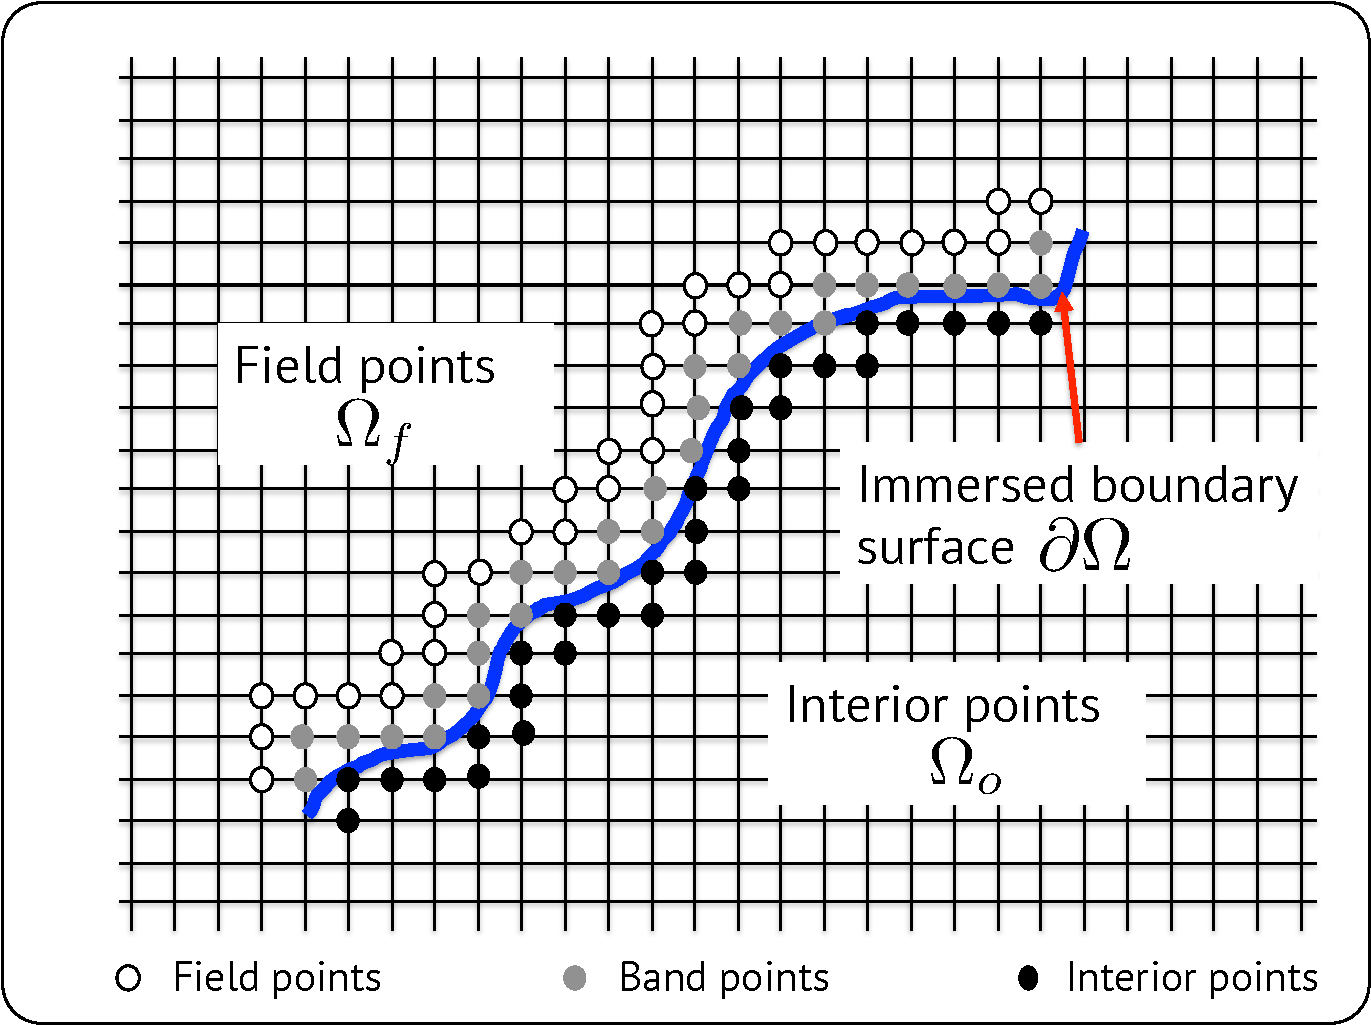
\includegraphics[scale=0.5]{fig/ib.pdf}
\caption{Mesh points for IB methods} \label{fig:ib_mesh}
\end{figure}
\item
Introducing so-called Mask function, typically denoted as $\chi(\mb x)$, which is nothing but indicator function
\begin{align*}
\chi(\mb x) = \fbrl{\begin{array}{cl}
1, & \md{if } \mb x \in \Omega_o \\
0, & \md{else.}
\end{array}}
\end{align*}
\item
Altering governing equations by adding forcing terms, so that boundary conditions at the obstacle surface are approximately satisfied, involving the $\chi(\mb x)$ above, so that equations in field points do not change.
\end{enumerate}
Additional forcing terms can be added either before the governing equations are discretized or after. This order determines the type of methods in IB methods family. Volume penalization (VP) is a subclass of IB methods where equations are altered before the discretization, therefore conceptually does not depend on numerical approach to be used.

Consider the following Navier-Stokes equations
\begin{align}
\fbrl{\begin{array}{ll}
\ds \frac {\pt \rho}{\pt t} + \frac {\pt \rho u_j}{\pt x_j} &= 0 \\
\ds \frac {\pt \rho u_i}{\pt t} + \frac {\pt \rho u_i u_j}{\pt x_j} + \frac {\pt p}{\pt x_i} + \frac {\pt \tau_{ij}}{\pt x_j} &= 0\\
\ds \frac {\pt \rho e}{\pt t} + \frac {\pt u_j \rbr{\rho e + p}}{\pt x_j} + \frac {\pt u_i \tau_{ij}}{\pt x_j} &= 0,
\end{array}}
\end{align}
along with constitutive equations for ideal gas that form a closed system.

Throughout entire writeup numerically more convenient form of the equations as described below will be used:
\begin{align}
\frac {\pt \vp}{\pt t} &= RHS, \label{eq:rhs}
\end{align}
where $RHS$ is different for each equation.

The idea behind the Brinkman penalization is to alter momentum equation, i.e. penalize it, at every grid point. 
\begin{align}
\frac {\pt \rho u_i}{\pt t} &= RHS - \frac \chi \eta {\rho \rbr{u_i - U_i^o}},
\end{align}
where $\eta$ is numerical permeability of the obstacle. One needs to keep in mind that it is artificial. This equation is unchanged outside of the obstacle due to the masking function and it mimics no slip boundary condition $u_i|_{\pt \Omega} = U_i^o$ at the timescale $\eta$. 

In order to reach proper acoustic reflection from the obstacle one can also introduce numerical porosity $\phi$ in continuity equation to mimic porous media in full extent.
\begin{align}
\nonumber
\frac {\pt \rho}{\pt t} &= -\frac 1\phi \frac {\pt \rho u_j}{\pt x_j},
\end{align}
which can be translated to the form \eqref{eq:rhs} as 
\begin{align}
\frac {\pt \rho}{\pt t} &= RHS - \chi \rbr{\frac 1\phi - 1} \frac {\pt \rho u_j}{\pt x_j}. \label{eq:poro_den}
\end{align}
One can also penalize temperature as well, in case such boundary condition is meant to be satisfied at the obstacle boundary.
\begin{align}
\frac {\pt T}{\pt t} &= RHS - \frac \chi \eta \rbr{T - T^o},
\end{align}
which mimics isothermal boundary condition $T|_{\pt \Omega} = T^o$ and can be incorporated to the energy equation through the full energy relation for ideal gas,
\begin{align}
\rho e &= \frac {\rho u_j u_j}2 + \rho c_VT = \frac {\rho u_j u_j}2 + \frac p{\gG - 1} \label{eq:igeos}.
\end{align}
Results of BPM implementation to supersonic inviscid flow are shown in Chapter 3 as a motivation for new VPM.

\section{Adaptive Wavelet Collocation Method}
For High Fidelity simulations to reduce number of used grid points, AWCM is used. Let us consider some target function $u(\mathbf x)$ that can be sampled on some uniform grid of chosen highest level of resolution, although grid does not have to be uniform, as long as it is structured. In this project uniform grid is used as a first step in grid adaptation. Following Vasilyev et al. \cite{lib:wlt_main} one can decompose given function into wavelet functions and scaling function at the lowest level of resolution
\begin{align}
u(\mathbf x) &= \sum_{k \in \mathcal K^0} c_k^0 \phi_k^0 (\mathbf x) + \sum_{j = 0}^\infty \sum_{\mu = 1}^{2^n - 1} \sum_{l \in \mathcal L^{\mu, j}} d_l^{\mu, j} \psi_l^{\mu, j} (\mathbf x),
\end{align}
where $\phi_k^0(\mathbf x)$ is a scaling function at the coarsest level of resolution and $\psi_l^{\mu, j}(\mathbf x)$ is a wavelet function at the level of resolution $j$, $c_k^0$ and $d_l^{\mu, j}$ are scaling and wavelet coefficients accordingly. Main advantage of the decomposition above is it can be split into two parts
\begin{align}
u(\mathbf x) &= u_\ge (\mathbf x) + u_< (\mathbf x),
\end{align}
where
\begin{align}
\nonumber
u_\ge (\mathbf x) &= \sum_{k \in \mathcal K^0} c_k^0 \phi_k^0 (\mathbf x) + \sum_{j = 0}^\infty \sum_{\mu = 1}^{2^n - 1} \sum_{\substack{l \in \mathcal L^{\mu, j} \\ \lbr{d_l^{\mu, j}} \ge \epsilon \dbr u }} d_l^{\mu, j} \psi_l^{\mu, j} (\mathbf x), \\
u_<(\mathbf x) &= \sum_{j = 0}^\infty \sum_{\mu = 1}^{2^n - 1} \sum_{\substack{l \in \mathcal L^{\mu, j} \\ \lbr{d_l^{\mu, j}} < \epsilon \dbr u }} d_l^{\mu, j} \psi_l^{\mu, j} (\mathbf x),
\end{align}
based on some threshold value $\ges$. Donoho \cite{lib:donoho} had shown that absolute error of neglecting $u_<(\mathbf x)$ part of the function leads to controllable error on the function, namely
\begin{align}
\dbr{u - u_\ge} \le C \ges \dbr u,
\end{align}
which means that one can use only part of the grid points and retain desired accuracy. This property allows to construct an adaptive grid with significantly fewer number of points. Only the regions with steep gradients have large values of wavelet coefficients, which makes wavelets a good indicator of those gradients. For example, in Fig.~\ref{fig:wlt_decomp} wavelet coefficients of the function with two sharp transitions are presented.

Wavelet basis functions possess other ``nice'' properties, such as localization in both space and time. In this project, along with all other projects conducted in Multiscale Modeling and Simulation Laboratory, interpolating wavelets are used (See Fig.~\ref{fig:wlt}). Constructing wavelet functions is relatively simple and have well described recursive algorithm \cite{lib:wlt_home}.

\begin{figure}[t]
\centering 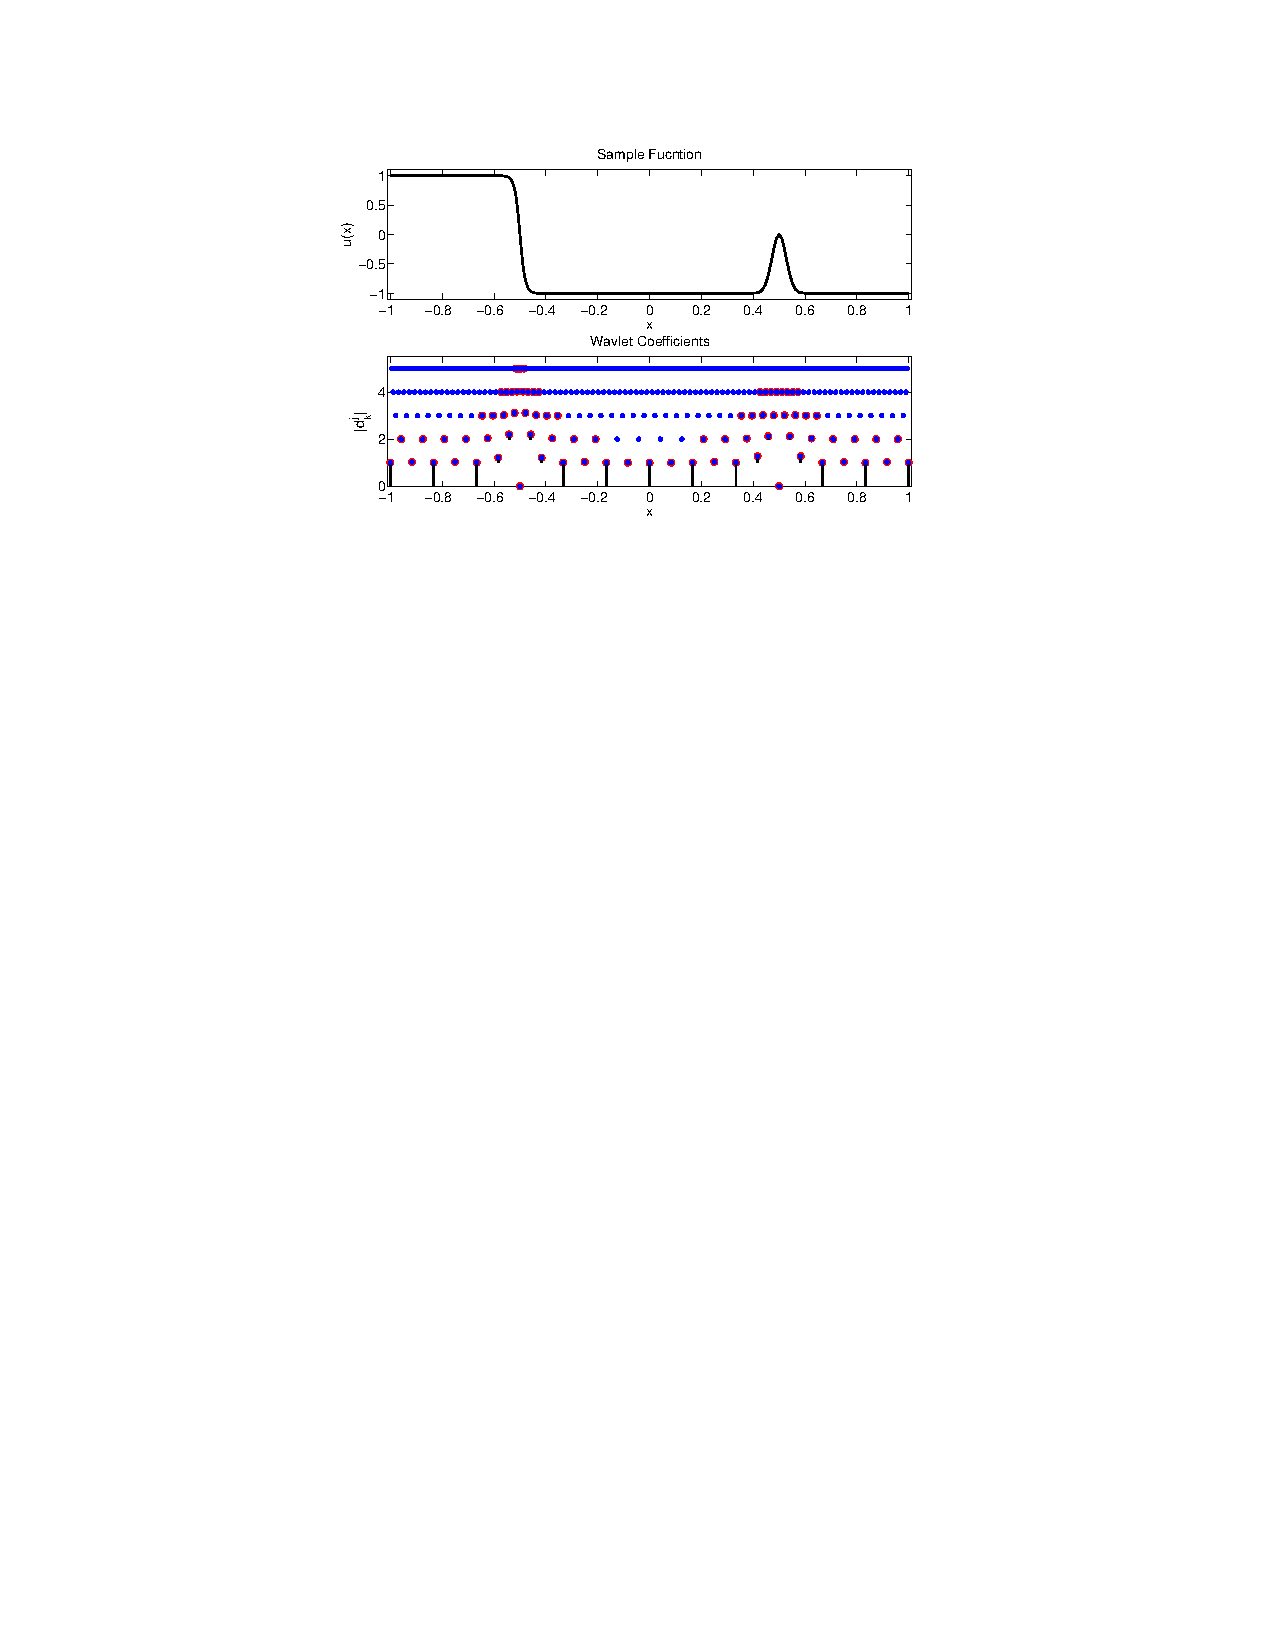
\includegraphics[scale=1]{fig/wlt_decomp.pdf}\\
\caption{Wavelet coefficients of a function with two sharp transitions \label{fig:wlt_decomp}}
\end{figure}
\begin{figure}[h!]
\begin{minipage}{0.5\linewidth}
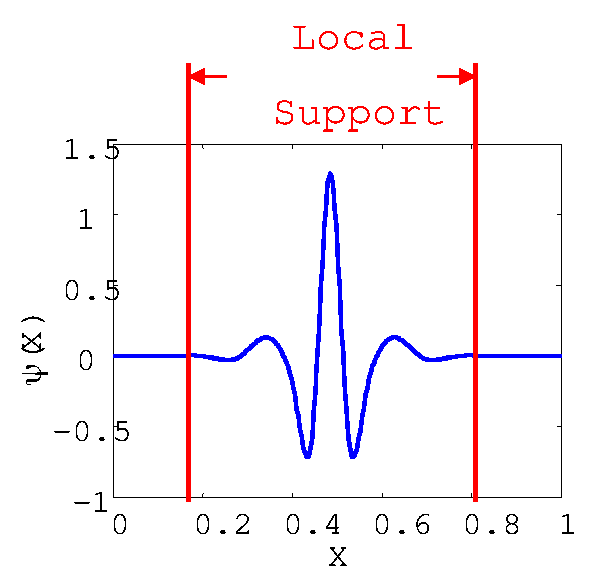
\includegraphics[scale=0.7]{fig/wlt.pdf}\\
\centering{a) Interpolating wavelet of 3$^{rd}$ order}
\end{minipage}
\begin{minipage}{0.5\linewidth}
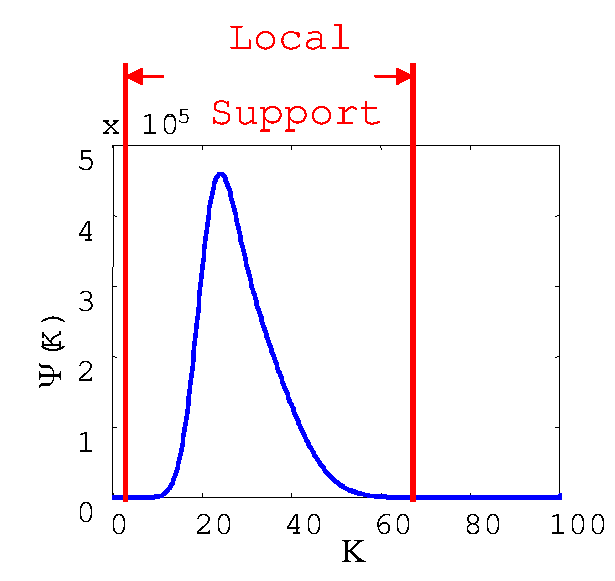
\includegraphics[scale=0.7]{fig/wlt_fft.pdf}\\
\centering{b) Fourier transform of wavelet}
\end{minipage}
\caption{Localized nature of wavelet function} \label{fig:wlt}
\end{figure}

Adaptation procedure can be easily iterated over time evolution, which makes it also a dynamic, so one can assure that grid always represents current state of the physical phenomenon. In order to do this properly the concept of Adjacent Zone is introduced \cite{lib:adjacent} (see Fig.~\ref{fig:wlt_adj}).
\begin{figure}[h!]
\centering 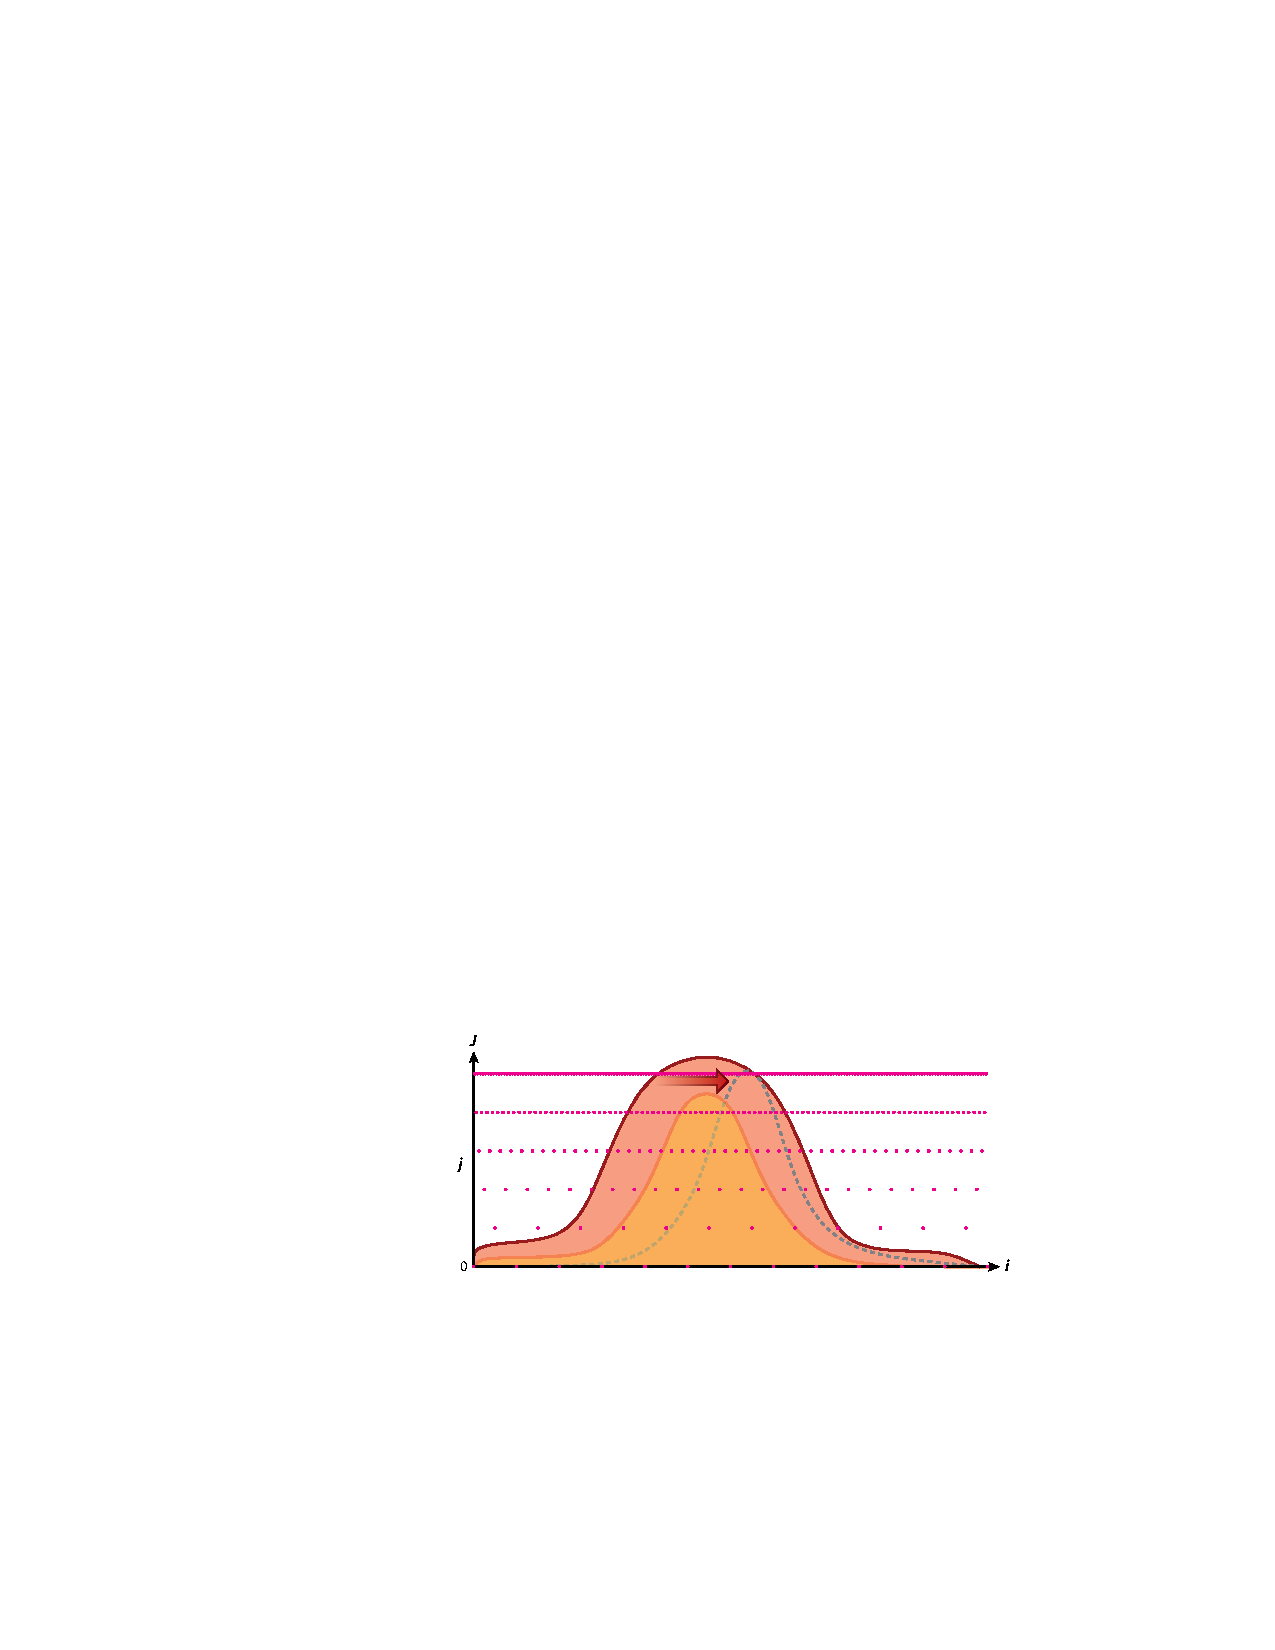
\includegraphics[scale=1]{fig/wlt_adj.pdf}\\
\caption{Safety region with possible significant wavelets after one time step \cite{lib:wlt_main} \label{fig:wlt_adj}}
\end{figure}\\
One may consider it as a safety regions within which coefficients might become significant even after the time integration. In this case one can make sure that global accuracy of the simulations is still within the user defined and controlled threshold in evolution problems, and most importantly keep adapted grid in up to date state. Using adapted grid also saves memory required to store variable values at each grid point, since one needs fewer of them.

\section{Wavelet Based Artificial Viscosity as a Shock Capturing Scheme}
Using AWCM becomes even more attractive for High Fidelity simulations per discussion in previous section --- Wavelet coefficients have large values at the regions of steep gradients and discontinuities are as steep as one can get. Numerically it means that there are coefficients on all levels of resolution. By Regele and Vasilyev \cite{lib:RegVas} is developed a method to track and smooth those gradients. The core of the method is to add artificial viscosity to the desired hyperbolic equation with dynamic artificial viscosity, when latter depends on ``shock locator'' --- specifically cooked flux limiting function. Let us consider simple one dimensional conservation equation with added artificial diffusion term,
\begin{align}
\frac {\pt u}{\pt t} + \frac {\pt f}{\pt x} &= \frac \pt {\pt x} \rbr{\nu \rbr{\Phi} \frac {\pt u}{\pt x}},
\end{align}
where $\Phi$ can be found as
\begin{align}
\Phi &= \fbrl{\begin{array}{ll}
\frac {\lbr{d_k^{j_{max}}}}{\dbr u}, & \md{if } 0 < \lbr{d_k^{j_{max}}} \le \ges_d \dbr u \\
1, & \md{if } \lbr{d_k^{j_{max}}} > \ges_d \dbr u,
\end{array}}
\end{align}
where $\lbr{d_k^{j_{max}}}$ is a wavelet coefficient at fines level of resolution and $\ges_d$ is also a chosen thresholding parameter to limit $\Phi$, apart from the wavelet threshold parameter $\ges$.

In Fig.~\ref{fig:visc} one may find viscosity field and corresponding Schlieren image of the density field for 2D supersonic flow around the solid circle. Problem is solved using aforementioned artificial viscosity. Per methods design, viscosity is non-zero at shock locations, based on the Schlieren image, and vanishes everywhere else.
\begin{figure}[h!]
\begin{minipage}{0.5\linewidth}
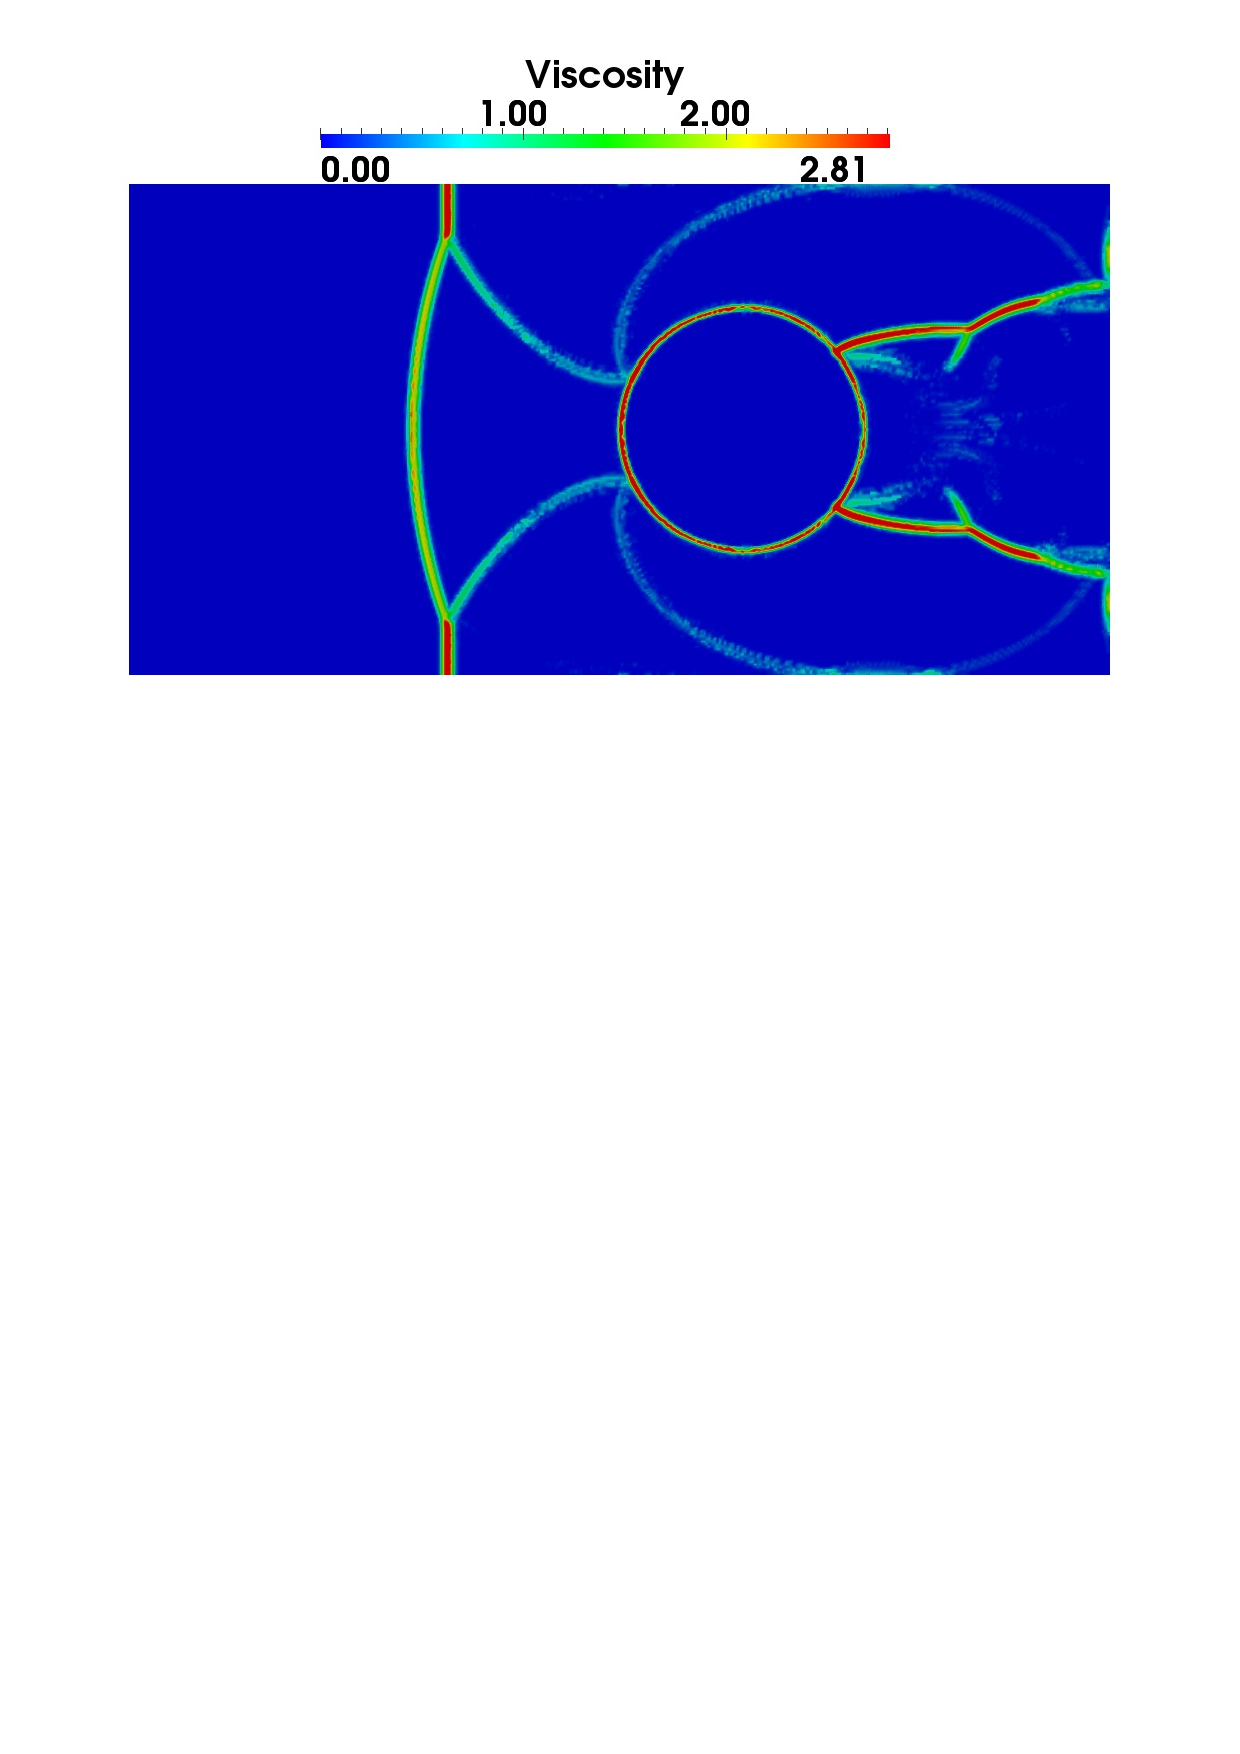
\includegraphics[scale=0.4]{fig/visc.pdf}\\
\centering{a) Viscosity field}
\end{minipage}
\begin{minipage}{0.5\linewidth}
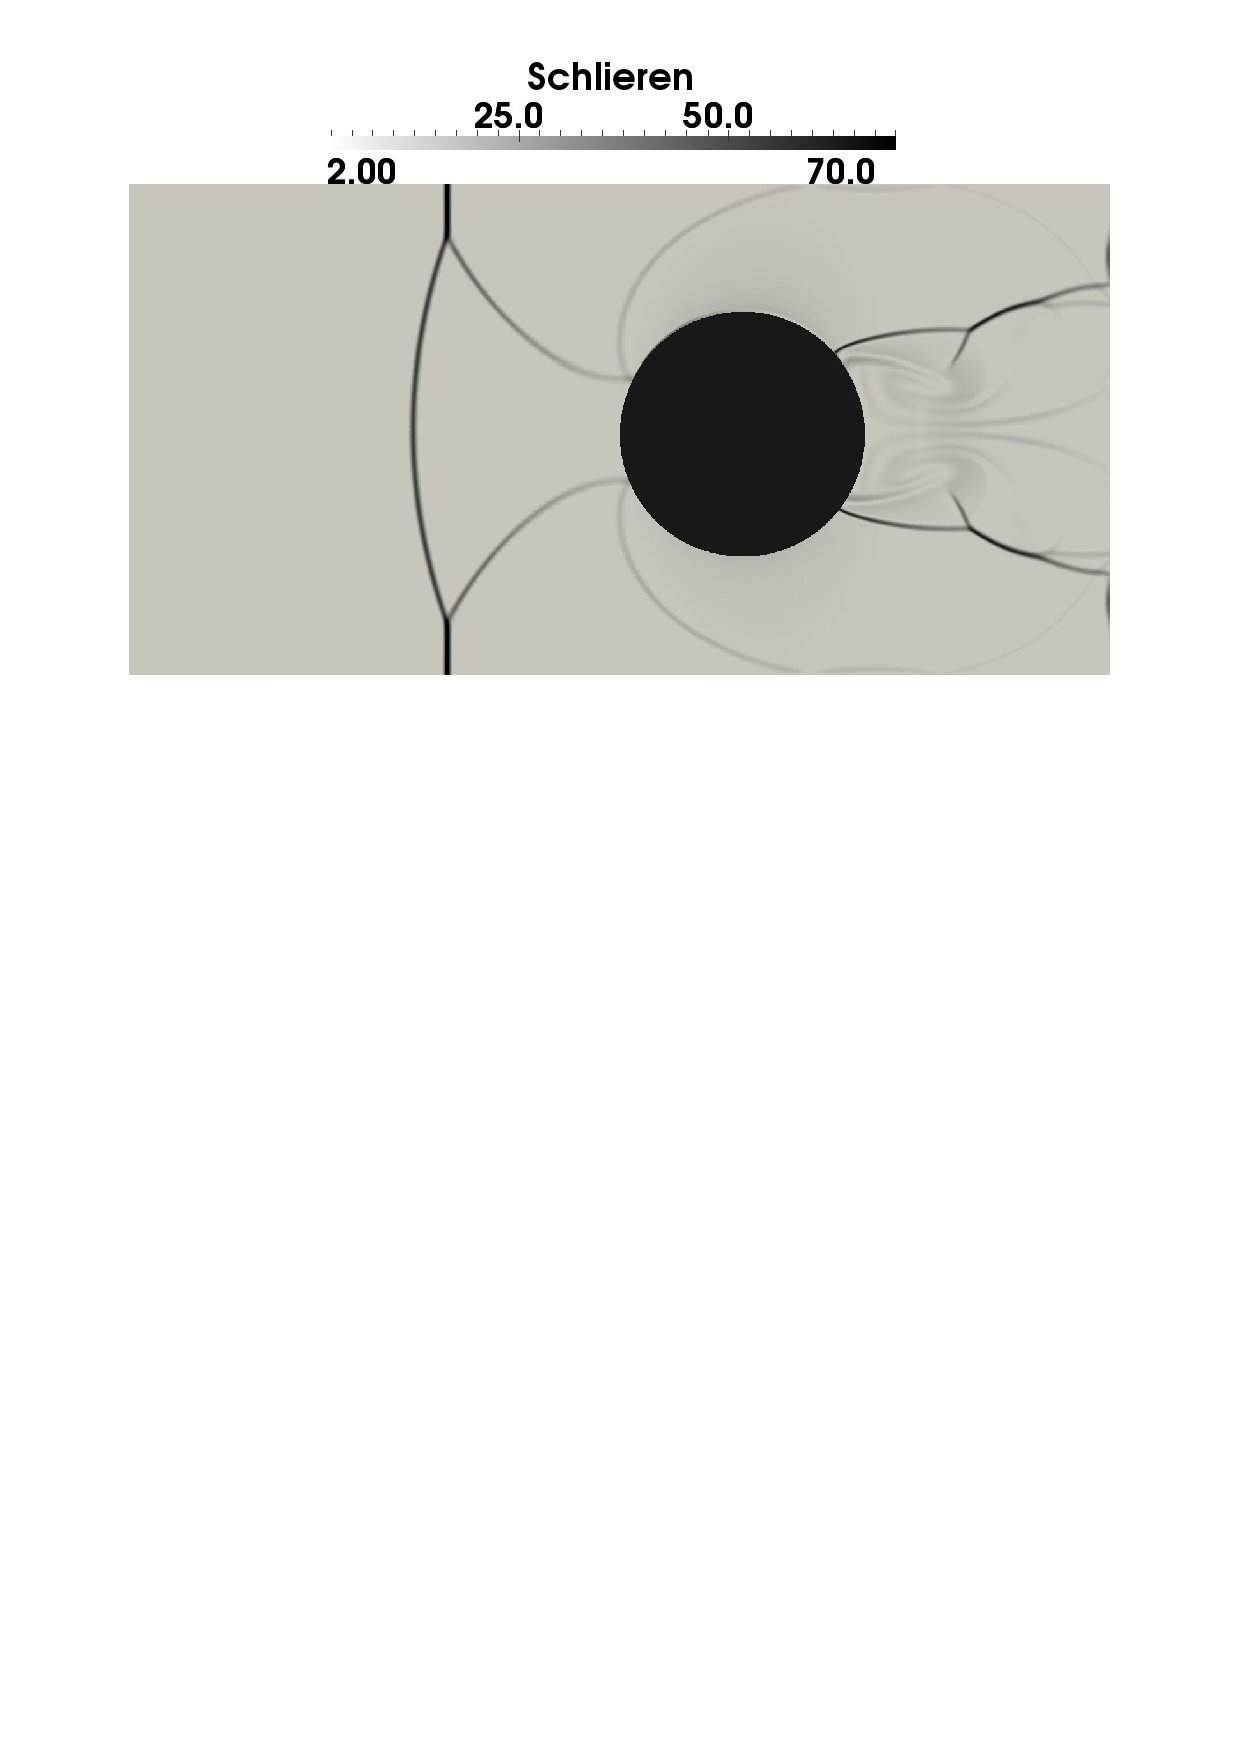
\includegraphics[scale=0.4]{fig/visc_sch.pdf}\\
\centering{b) Schlieren image of the flow}
\end{minipage}
\caption{Localized nature of wavelet function} \label{fig:visc}
\end{figure}

\section{Riemann Problem and Riemann Solver of Roe}
A Riemann problem consists of a conservation laws together with piecewise constant data having a single discontinuity, or in other words, one or multiple hyperbolic equations with discontinuous initial conditions. As a such system one can consider Euler or Navier-Stokes equations. Either numerical or analytical technique to solve such a problem is called Riemann solver. For non-linear problems, like Euler and Navier-Stokes, there are number of numerical Riemann solvers, such as Godunov Scheme, Flux Vector Splitting, Roe solver \cite{book:Toro}, etc. For Low Fidelity simulations of this project latter is used.

For the sake of simplicity, let us consider pseudo one dimensional Euler equations for ideal gas with discontinuous ICs.
\begin{align}
\nonumber
\frac {\pt \mathbf u}{\pt t} + \frac {\pt \mathbf F \rbr{\mathbf u}}{\pt x} = 0 \\
\mathbf u = \fbrl{\begin{array}{ll}
\mathbf u_L, & \md{if } x \le x_S \\
\mathbf u_R, & \md{if } x > x_S,
\end{array}}
\end{align}
where 
\begin{align}
\mathbf u = \sbr{\begin{array}{c}\rho \\ \rho u \\ \rho v \\ \rho w \\ \rho e \end{array}}, \qquad \mathbf F = \sbr{\begin{array}{c}\rho u \\ \rho u^2 + p \\ \rho uv \\ \rho u w \\ u \rbr{\rho e + p}\end{array}},
\end{align}
and constitutive equation \eqref{eq:igeos} to close the system. It can be rewritten in pseudo linear form
\begin{align}
\frac {\pt \mathbf u}{\pt t} + \mathcal A \rbr{\mathbf u}\frac {\pt \mathbf u}{\pt x} = 0, \label{eq:Euler}
\end{align}
where $\mathcal A$ is a Jacobian matrix of the flux $\mathbf F$ with respect to the solution vector $\mathbf u$, which has the following explicit relation
\begin{align}
\mathcal A = \sbr {\begin{array}{ccccc}
0 & 1 & 0 & 0 & 0 \\
\hat \gG H - u^2 - a^2 & (3-\gG)u & -\hat \gG v  & -\hat \gG w & \hat \gG \\
-u v & v & u & 0 & 0 \\
-u w & w & 0 & u & 0 \\
u \sbr{(\gG - 2)H - a^2} & H - \hat \gG u^2 & - \hat \gG u v & - \hat \gG u w & \gG u
\end{array}}, \label{eq:matrix}
\end{align}
where $\hat \gG = \gG - 1$, $H = (\rho e + p)/\rho$ (Specific enthalpy) and $a = \sqrt{\gG p / \rho}$ (Local speed of sound). This matrix has eigenvalues 
\begin{align}
\gl_1 = u - a, \quad \gl_2 = \gl_3 = \gl_4 = u, \quad \gl_5 = u + a,
\end{align}
and eigenvectors
\begin{align}
\fbrr{\begin{array}{c}
\mathbf K^{(1)} = \sbr{\begin{array}{c}
1 \\ u - a \\ v \\ w \\ H - ua
\end{array}}, \mathbf K^{(2)} = \sbr{\begin{array}{c}
1 \\ u  \\ v \\ w \\ \frac 12 V^2
\end{array}}, \mathbf K^{(3)} = \sbr{\begin{array}{c}
0 \\ 0 \\ 1 \\ 0 \\ v
\end{array}}, \\
\mathbf K^{(4)} = \sbr{\begin{array}{c}
0 \\ 0 \\ 0 \\ 1 \\ w
\end{array}}, \mathbf K^{(5)} = \sbr{\begin{array}{c}
1 \\ u + a \\ v \\ w \\ H + ua
\end{array}}
\end{array}}, \label{eq:eigenvecs}
\end{align}
where $V = \rbr{u^2+v^2+w^2}$.

Equation \eqref{eq:Euler} can be numerically integrated as
\begin{align}
\mathbf u_i^{n+1} = \mathbf u_i^n + \frac {\gD t}{\gD x} \rbr{\mathbf F_{i - \frac 12} - \mathbf F_{i + \frac 12}},
\end{align}
where half-integer indices are introduced for convenience and to distinguish intercell values from cell values on chosen grid. Variety of Riemann solvers differ by the way they calculate those intercell values.

Philip Roe proposed to calculate intercell fluxes using certain averaging procedure based on right and left values of corresponding local fluxes \cite{lib:Roe} as follows
\begin{align}
\begin{array}{c}
\widetilde {\rbr \bullet} = \ds \frac {\sqrt {\rho_L} \rbr \bullet_L + \sqrt {\rho_R} \rbr \bullet_R}{\sqrt{\rho_L} + \sqrt{\rho_R}}
\end{array},
\end{align}
where $\rbr \bullet$ stands for $u, v, w$ and $H$. After finding these averaged values, one also needs to find $\widetilde V$ and $\widetilde a$ as 
\begin{align*}
\widetilde V &= \widetilde u^2 + \widetilde v^2 + \widetilde w^2, \\
\widetilde a &= \sbr{\hat \gG \rbr{\widetilde H - \frac 12 \widetilde V^2}}^{\frac 12}.
\end{align*}
Next step is to substitute all values defined in \eqref{eq:matrix}-\eqref{eq:eigenvecs} with averaged values. Finally, according to Roe, intercell flux can be found as
\begin{align}
\mathbf F_{i+\frac 12} = \frac 12 \rbr{\mathbf F_L + \mathbf F_R} - \frac 12 \sum_{j = 1}^5 	\widetilde \ga_j \lbr{\widetilde \gl_j} \widetilde {\mathbf K^j},
\end{align}
where $\ga_j$ is so called wave strength --- weight that takes into account contribution from each eigenvector. Roe's original approach is to calculate them as follows:
\begin{align}
\nonumber
\widetilde \ga_3 &= \gD u_3 - \widetilde v \gD u_1, \\
\nonumber
\widetilde \ga_4 &= \gD u_4 - \widetilde w \gD u_1, \\
\widetilde \ga_2 &= \frac {\hat \gG}{\widetilde a^2} \sbr{\gD u_1 \rbr{\widetilde H - \widetilde u^2} + \widetilde u \gD u_2 - \overline{\gD u_5}}, \\
\nonumber
\widetilde \ga_1 &= \frac 1{2 \widetilde a} \sbr{\gD u_1 \rbr{\widetilde u + \widetilde a} - \gD u_2 - \widetilde a \widetilde \ga_2}, \\
\nonumber
\widetilde \ga_5 &= \gD u_1 - \rbr{\widetilde \ga_1 + \widetilde \ga_2},
\end{align}
where $\gD \mathbf u = \mathbf u_R - \mathbf u_L$ and $\overline{\gD u_5} = \gD u_5 - \widetilde \ga_3 \widetilde v - \widetilde \ga_4 \widetilde w$. $\mathbf u$ --- is a solution vector. This procedure can be naturally extended to the full 3D case, with simple directional rotation of coordinate system and considering each direction as flow direction in pseudo one dimensional problem.





